\documentclass{article}
\usepackage[UTF8]{ctex}
\usepackage{pythonhighlight}
\usepackage{markdown}
\usepackage{listings}
\lstset{
    basicstyle          =   \tt,          % 基本代码风格
    identifierstyle=\color{brown!80!black},
    keywordstyle        =   \color{purple}\bfseries,          % 关键字风格
    commentstyle        =   \rmfamily\itshape,  % 注释的风格,斜体
    stringstyle         =   \ttfamily,  % 字符串风格
    flexiblecolumns,                % 别问为什么,加上这个
    numbers             =   left,   % 行号的位置在左边
    showspaces          =   false,  % 是否显示空格,显示了有点乱,所以不现实了
    numberstyle         =   \zihao{-5}\ttfamily,    % 行号的样式,小五号,tt等宽字体
    showstringspaces    =   false,
    captionpos          =   t,      % 这段代码的名字所呈现的位置,t指的是top上面
    frame               =   lrtb,   % 显示边框
    backgroundcolor=\color[RGB]{245,245,244},
}


% Language setting
% Replace `english' with e.g. `spanish' to change the document language
\usepackage[english]{babel}
\usepackage{float}
% Set page size and margins
% Replace `letterpaper' with `a4paper' for UK/EU standard size
\usepackage[letterpaper,top=2cm,bottom=2cm,left=3cm,right=3cm,marginparwidth=1.75cm]{geometry}

% Useful packages
\usepackage{amsmath}
\usepackage{graphicx}
\usepackage[colorlinks=true, allcolors=blue]{hyperref}

\title{普物虚拟实验报告3}
\author{雷远航 \ 学号:3210105807}

\begin{document}

\maketitle

\begin{abstract}
    热敏电阻温度特性研究
\end{abstract}

\section*{一、实验目的}
\subsubsection*{- 了解热敏电阻的电阻——温度特性及测温原理}
\subsubsection*{- 惠斯登电桥原理及使用方法}
\subsubsection*{- 学习作图法进行数据处理}



\section*{二、实验原理}

\subsection*{热敏电阻温度特性}
热敏电阻是一种传感器电阻,按照温度系数不同分为正温度系数热敏电阻器
(PTC)和负温度系数热敏电阻器(NTC)。正温度系数热敏电阻器(PTC)在温度
越高时电阻值越大,负温度系数热敏电阻器(NTC)在温度越高时电阻值越低。热
敏电阻的电阻值,随着温度的变化而改变,通过电阻的变化,电阻两端的电压就
会变化,所以可以用来制作感知温度变化的传感器。在微波炉上,它能够实时监测
内部的温度,因为热敏电阻对温度极为敏感,如果没有它,微波炉里面会出现过
热现象,那么就可能造成火灾的等人为灾害。

半导体热敏电阻的基本特性是它的温度特性,而这种特性是与
半导体材料的导电机制密切相关的。对于负温度系数热敏电阻,由
于半导体中的载流子数目随温度升高而按指数规律迅速增加,温度
越高,载流子的数目越多,导电能力越强,电阻率也就越小。因此
负温度系数热敏电阻随着温度的升高,它的电阻将按指数规律迅速
减小。

\subsection*{热敏电阻公式:}


\begin{figure}[H]
    \centering
    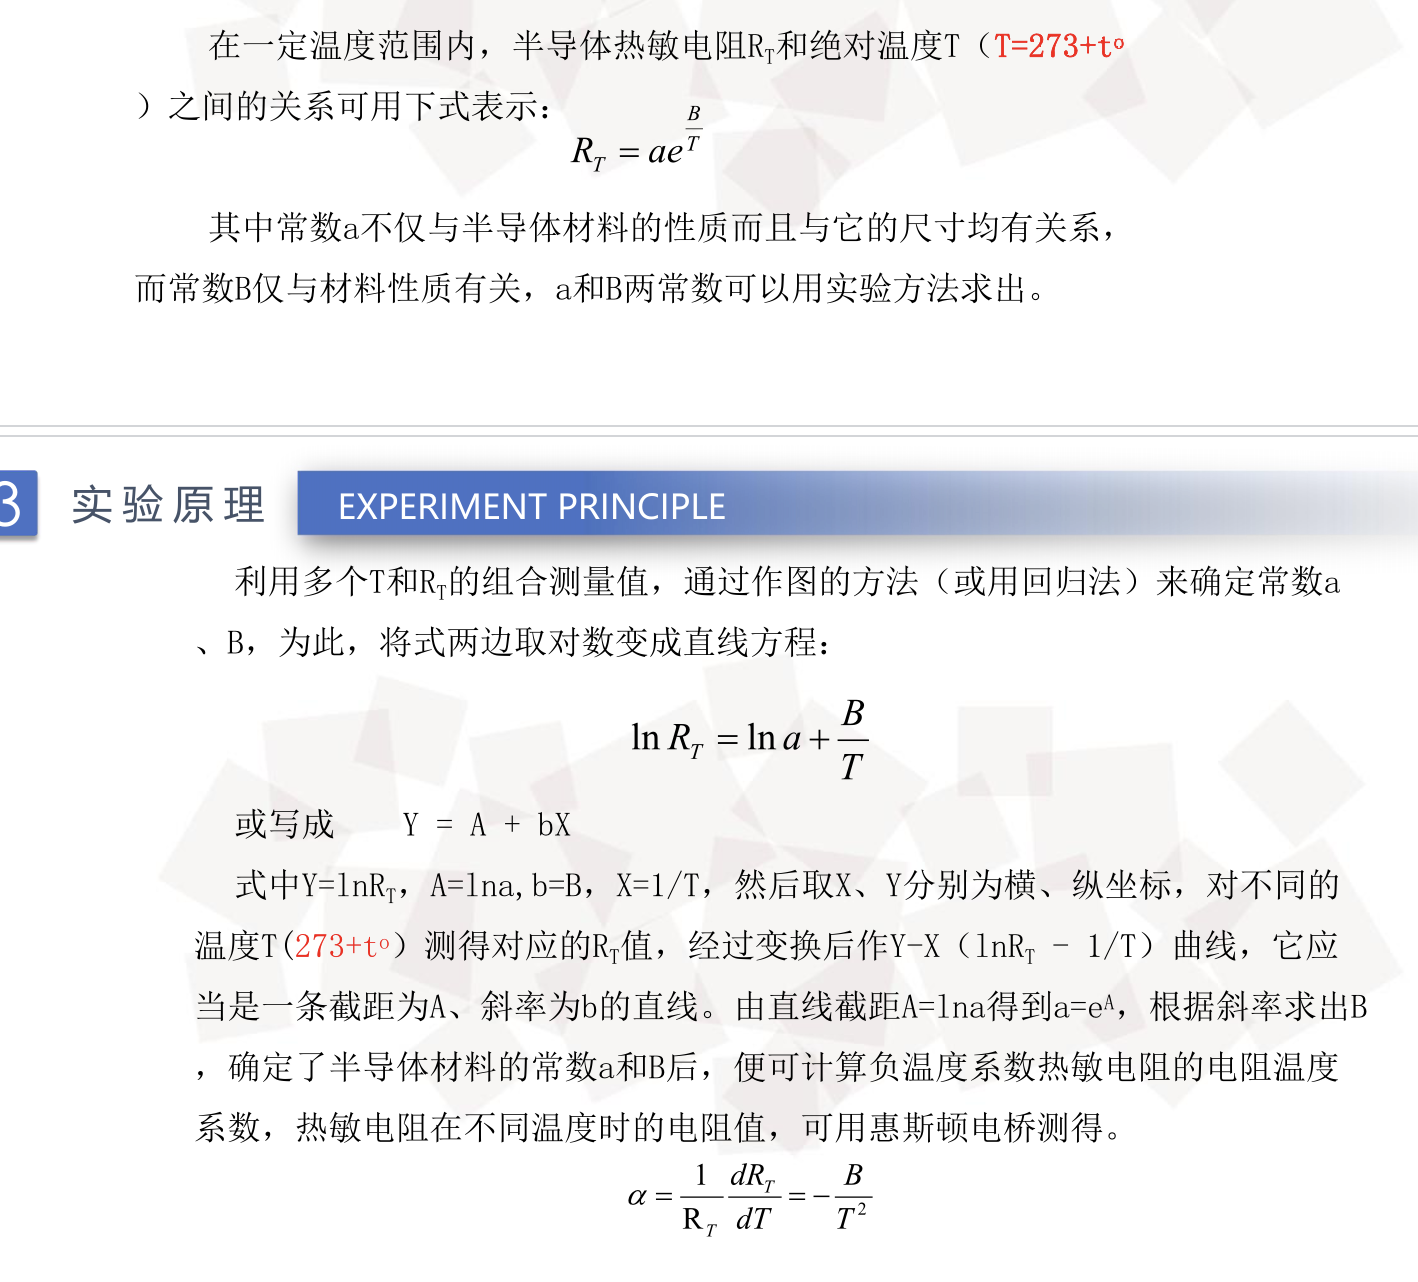
\includegraphics[width=0.7\textwidth]{2.png}

\end{figure}

\subsection*{惠斯登电桥}

\begin{figure}[H]
    \centering
    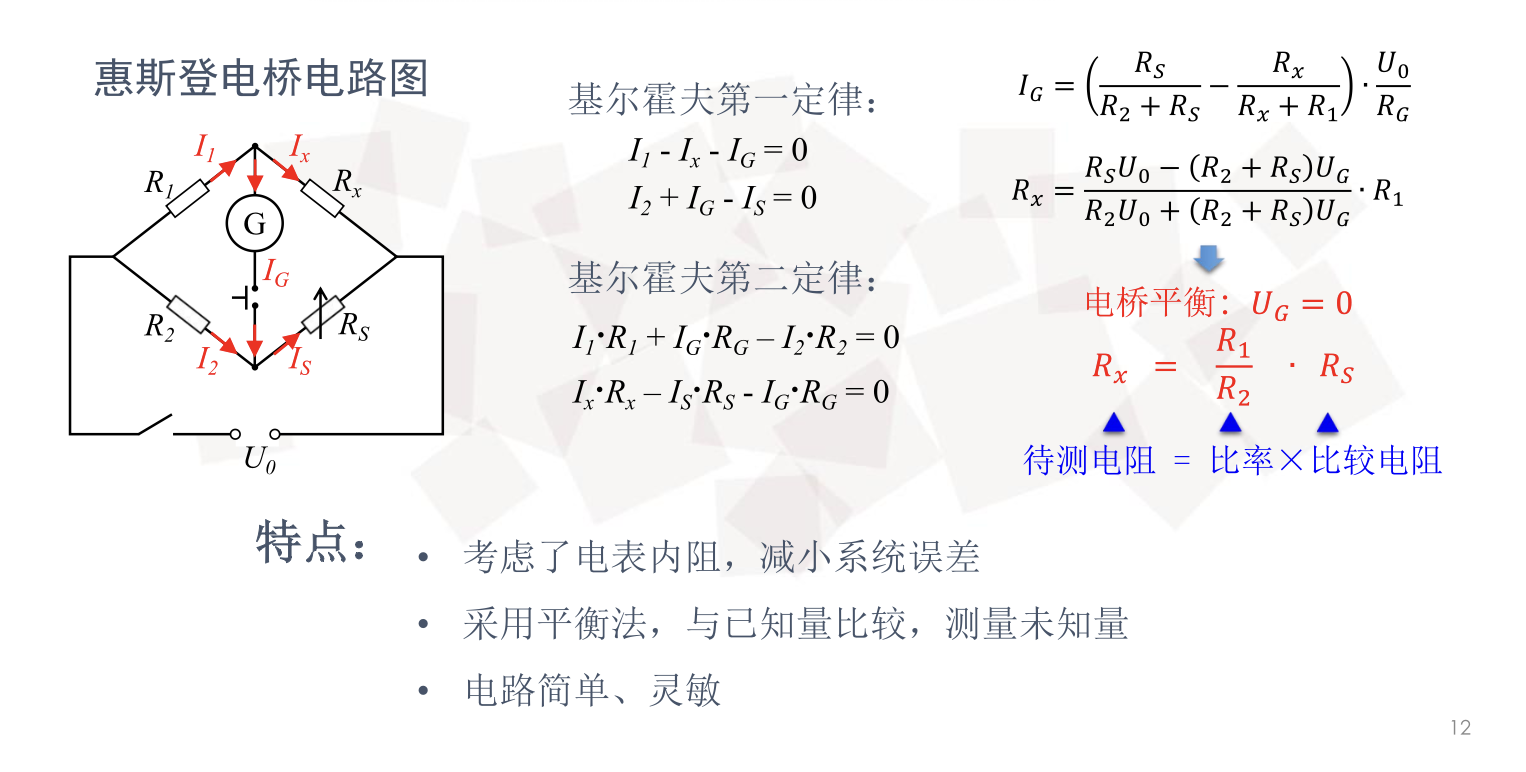
\includegraphics[width=0.7\textwidth]{3.png}

\end{figure}

\subsection*{电桥灵敏度}

\begin{figure}[H]
    \centering
    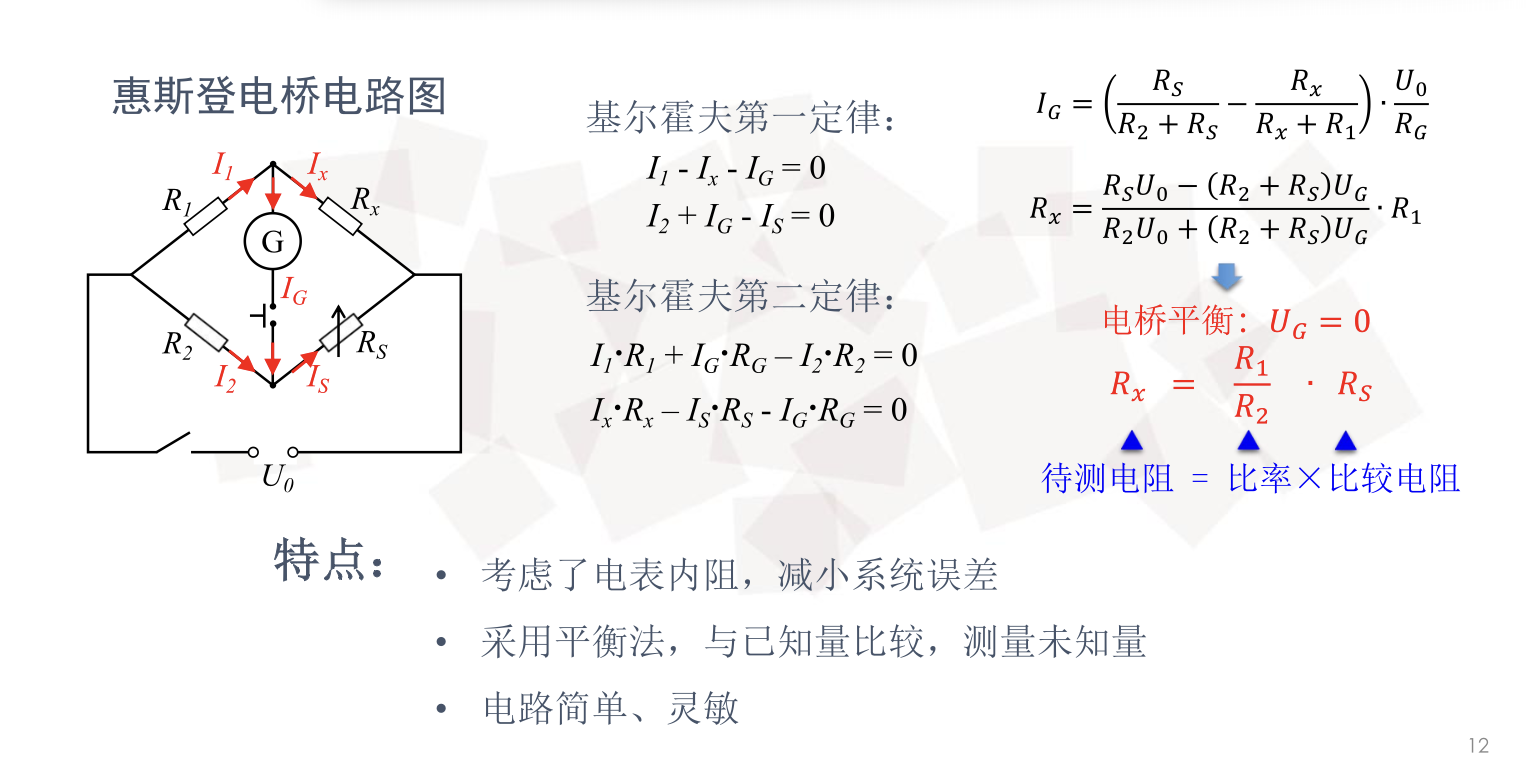
\includegraphics[width=0.7\textwidth]{4.png}
    
\end{figure}

电桥灵敏度分别为(截图中的有效数字不准确):28.8、 30.7、30.7

电桥灵敏度的平均值:30.0




    

\section*{三、实验内容}
\subsection*{1.用箱式电桥研究热敏电阻温度特性}
(1)使用内接电源和内接检流计,按照实验电路图连线。

(2)线路连接好以后,检流计调零。

(3)调节直流电桥平衡。

(4)测量并计算出室温时待测热敏电阻值Rx,微调电路中的电阻箱,测量并根据电桥灵敏度公
式:S=△n/(△Rx/Rx)或S=△n/(△R0/R0),计算出室温时直流电桥的电桥灵敏度。

(5)调节适当的自耦调压器输出电压值,使烧杯中的水温从20℃升高到85℃以上,每隔5℃测
量一次热敏电阻值Rt;再将自耦调压器输出电压值调为0V,使水慢慢冷却,降温过程中每隔
5℃测量一次热敏电阻值Rt,最终求取升降温的平均电阻值,并作出热敏电阻阻值与温度对应
关系曲线。

(6)根据测量结果,利用公式分别求取温度T趋于无穷时的热敏电阻阻值R∞、热敏电阻的材料
常数B以及50℃时的电阻温度系数α。

\subsection*{2.用自组式电桥研究热敏电阻温度特性}

(1)按实验电路图正确连线。

(2)线路连接好以后,检流计调零。

(3)调节直流电桥平衡。

(4)测量并计算出室温时待测热敏电阻值Rx,微调电路中的电阻箱,测量并根据电桥灵敏度公
式:S=△n/(△Rx/Rx)或S=△n/(△R0/R0),计算出室温时直流电桥的电桥灵敏度。

(5)选择合适的自耦调压器输出电压值,使烧杯中的水温从20℃升高到85℃以上,每隔5℃测
量一次热敏电阻阻值;再将自耦调压器输出电压值调为0V,在水温的从85℃下降到室温的过
程中,每隔5℃测量一次热敏电阻阻值,最终求取升降温的平均电阻值,并作出热敏电阻阻值
与温度对应关系曲线。

(6)根据测量结果,求取温度T趋于无穷时的热敏电阻阻值R∞、热敏电阻的材料常数B以及
50℃时的电阻温度系数α。


\section*{四、实验数据}
\subsection*{箱式电桥研究热敏电阻温度特性}
\subsubsection*{连接电路并且调节平衡:}
\begin{figure}[H]
    \centering
    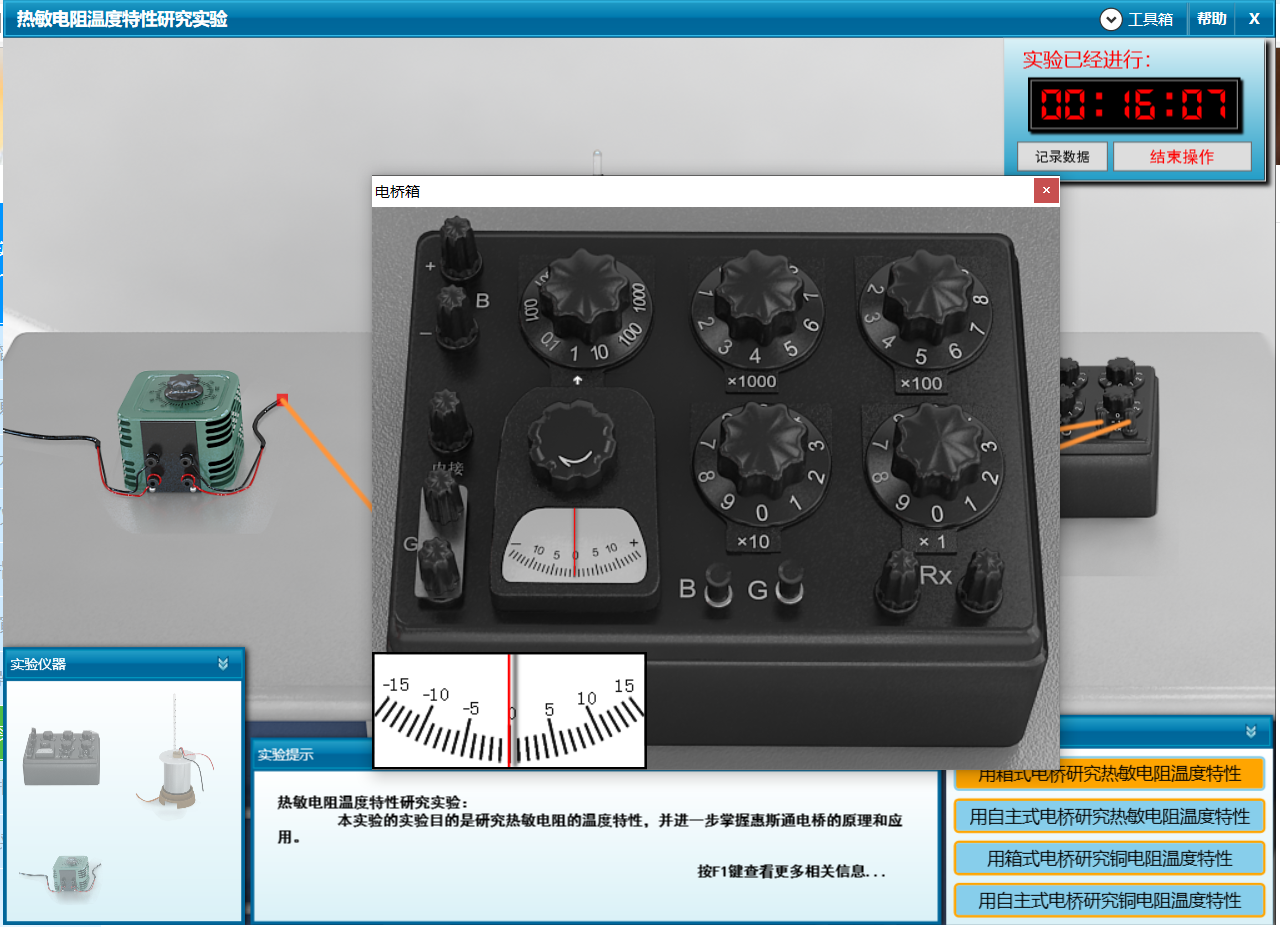
\includegraphics[width=0.7\textwidth]{虚拟3/1.png}
    
\end{figure}

\subsection*{计算电桥灵敏度}
对实验数据进行记录
\begin{figure}[H]
    \centering
    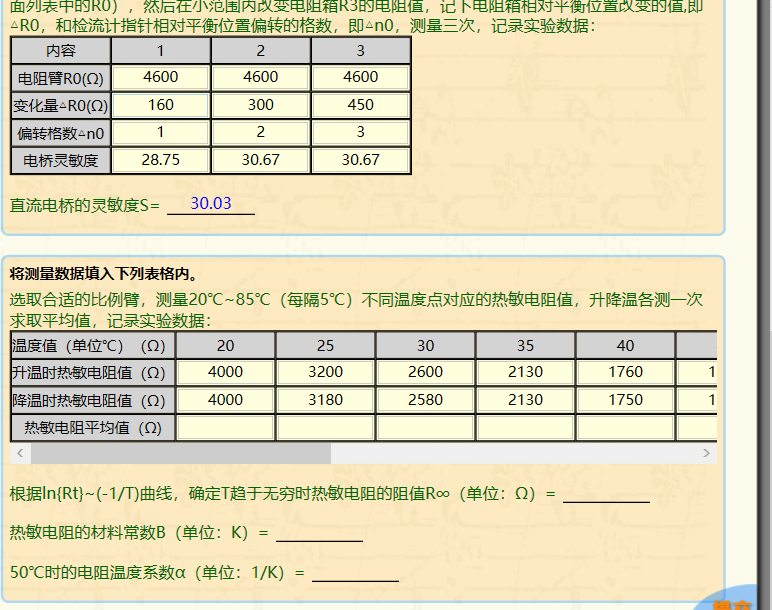
\includegraphics[width=0.7\textwidth]{虚拟3/4.png}
    
\end{figure}

电桥灵敏度分别为(截图中的有效数字不准确):30.0、 28.1、25.0

电桥灵敏度的平均值:27.7

\subsection*{温度系数计算}
用excel对数据进行处理
\begin{figure}[H]
    \centering
    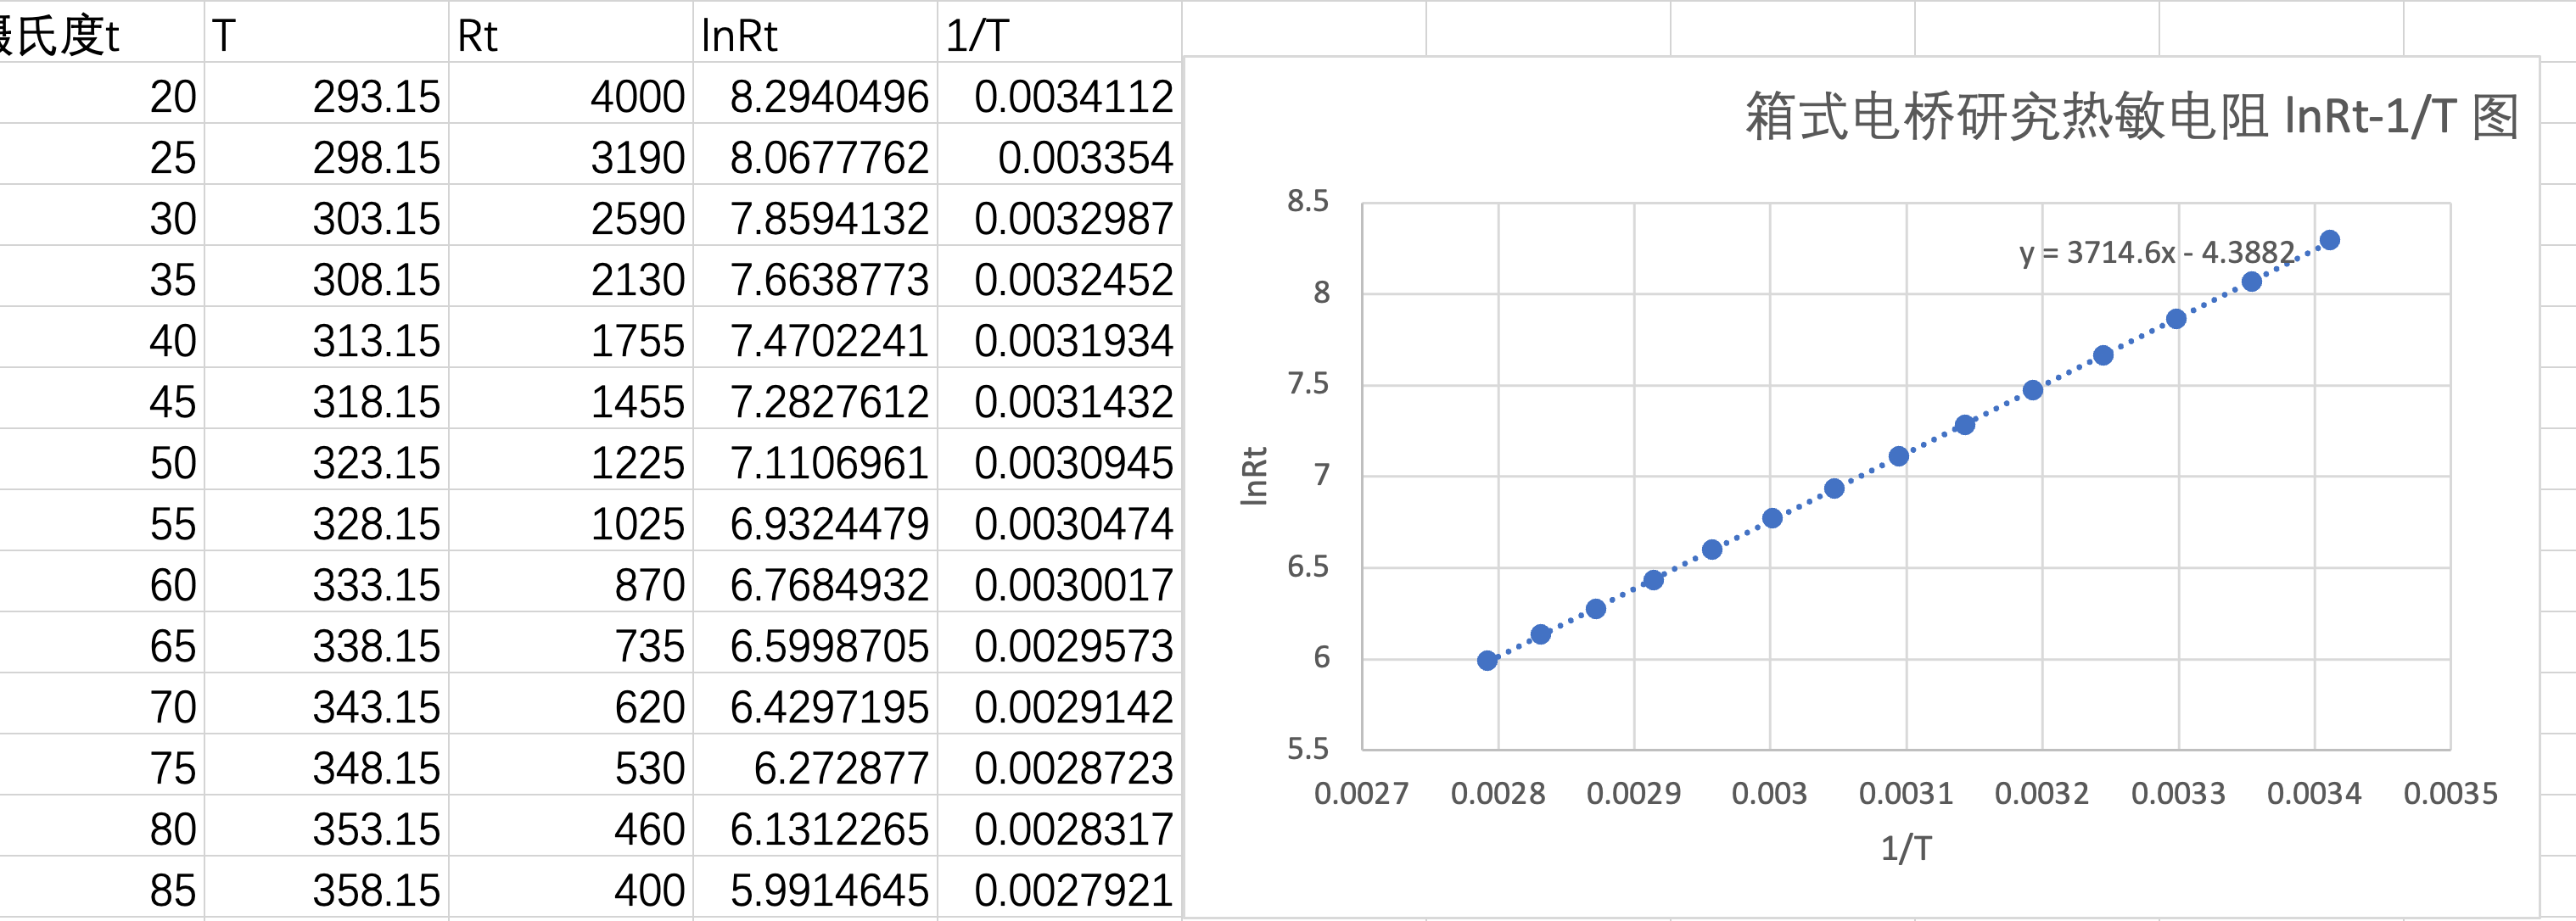
\includegraphics[width=0.9\textwidth]{5.png}
\end{figure}
(1)确定T趋于正无穷时热敏电阻的值:

截距A=-4.3882, 由:lna=A,  计算得:a=0.01243$\Omega$

(2)热敏电阻的材料常数B(单位:K):

材料常数B为拟合曲线的斜率:3714.6

(3)50摄氏度时的电阻温度系数$\alpha$(单位:1/K):

50+273.15=323.15K
由$\alpha=-\frac{B}{T^{2}}$=-0.0355



\subsection*{自组式电桥研究热敏电阻温度特性:}
\subsubsection*{对电路进行连接:}
\begin{figure}[H]
    \centering
    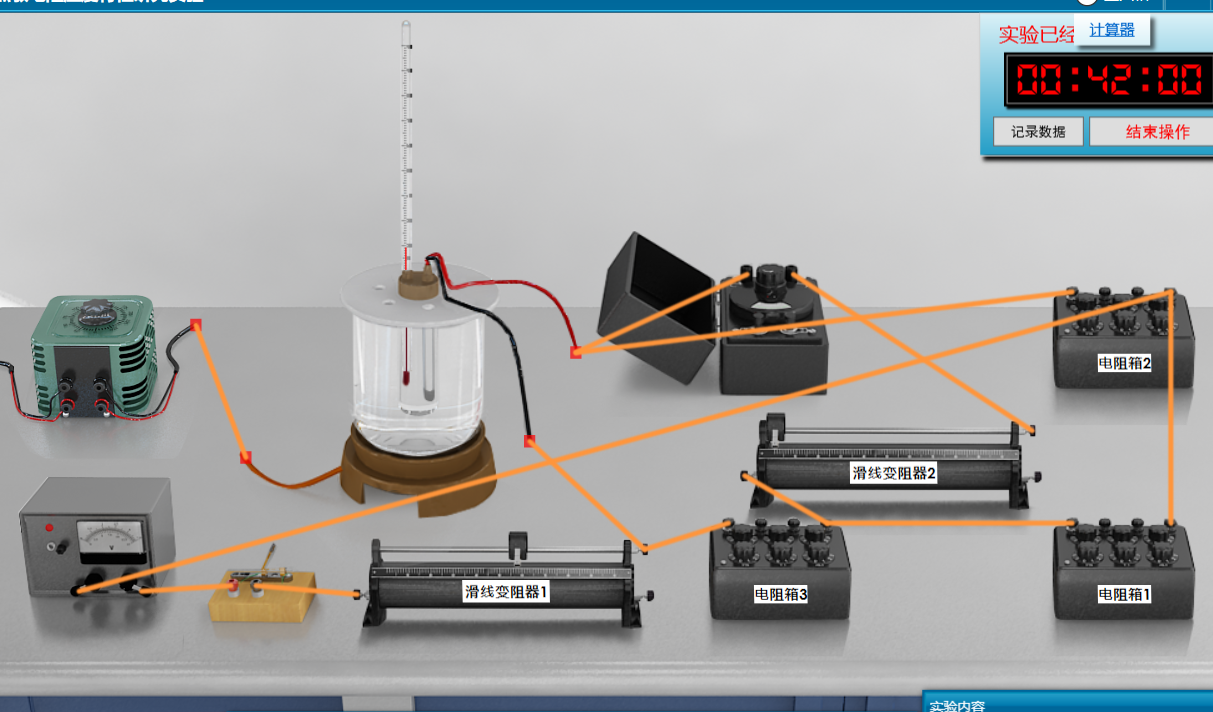
\includegraphics[width=0.9\textwidth]{虚拟3/5.png}
\end{figure}

\subsubsection*{计算电桥灵敏度:}
实验数据记录
\begin{figure}[H]
    \centering
    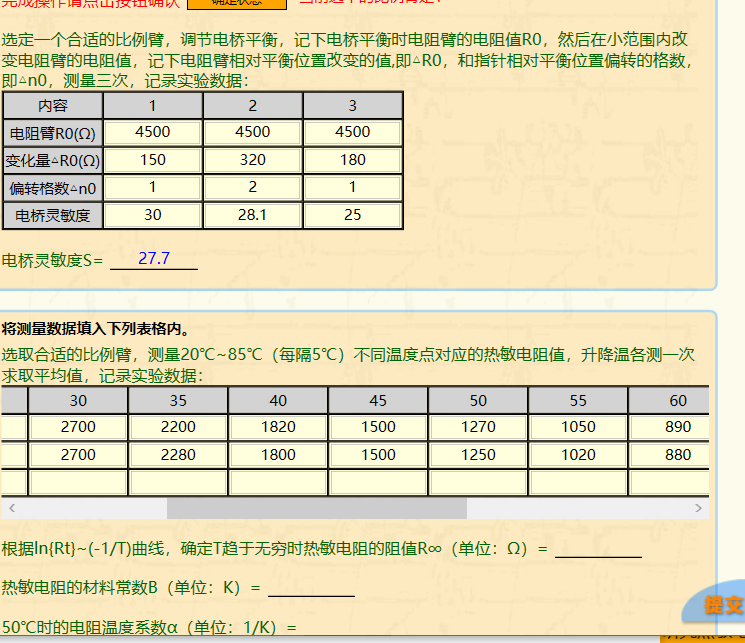
\includegraphics[width=0.7\textwidth]{虚拟3/3.png}
\end{figure}

\subsubsection*{温度系数计算:}

Excel进行数据处理
\begin{figure}[H]
    \centering
    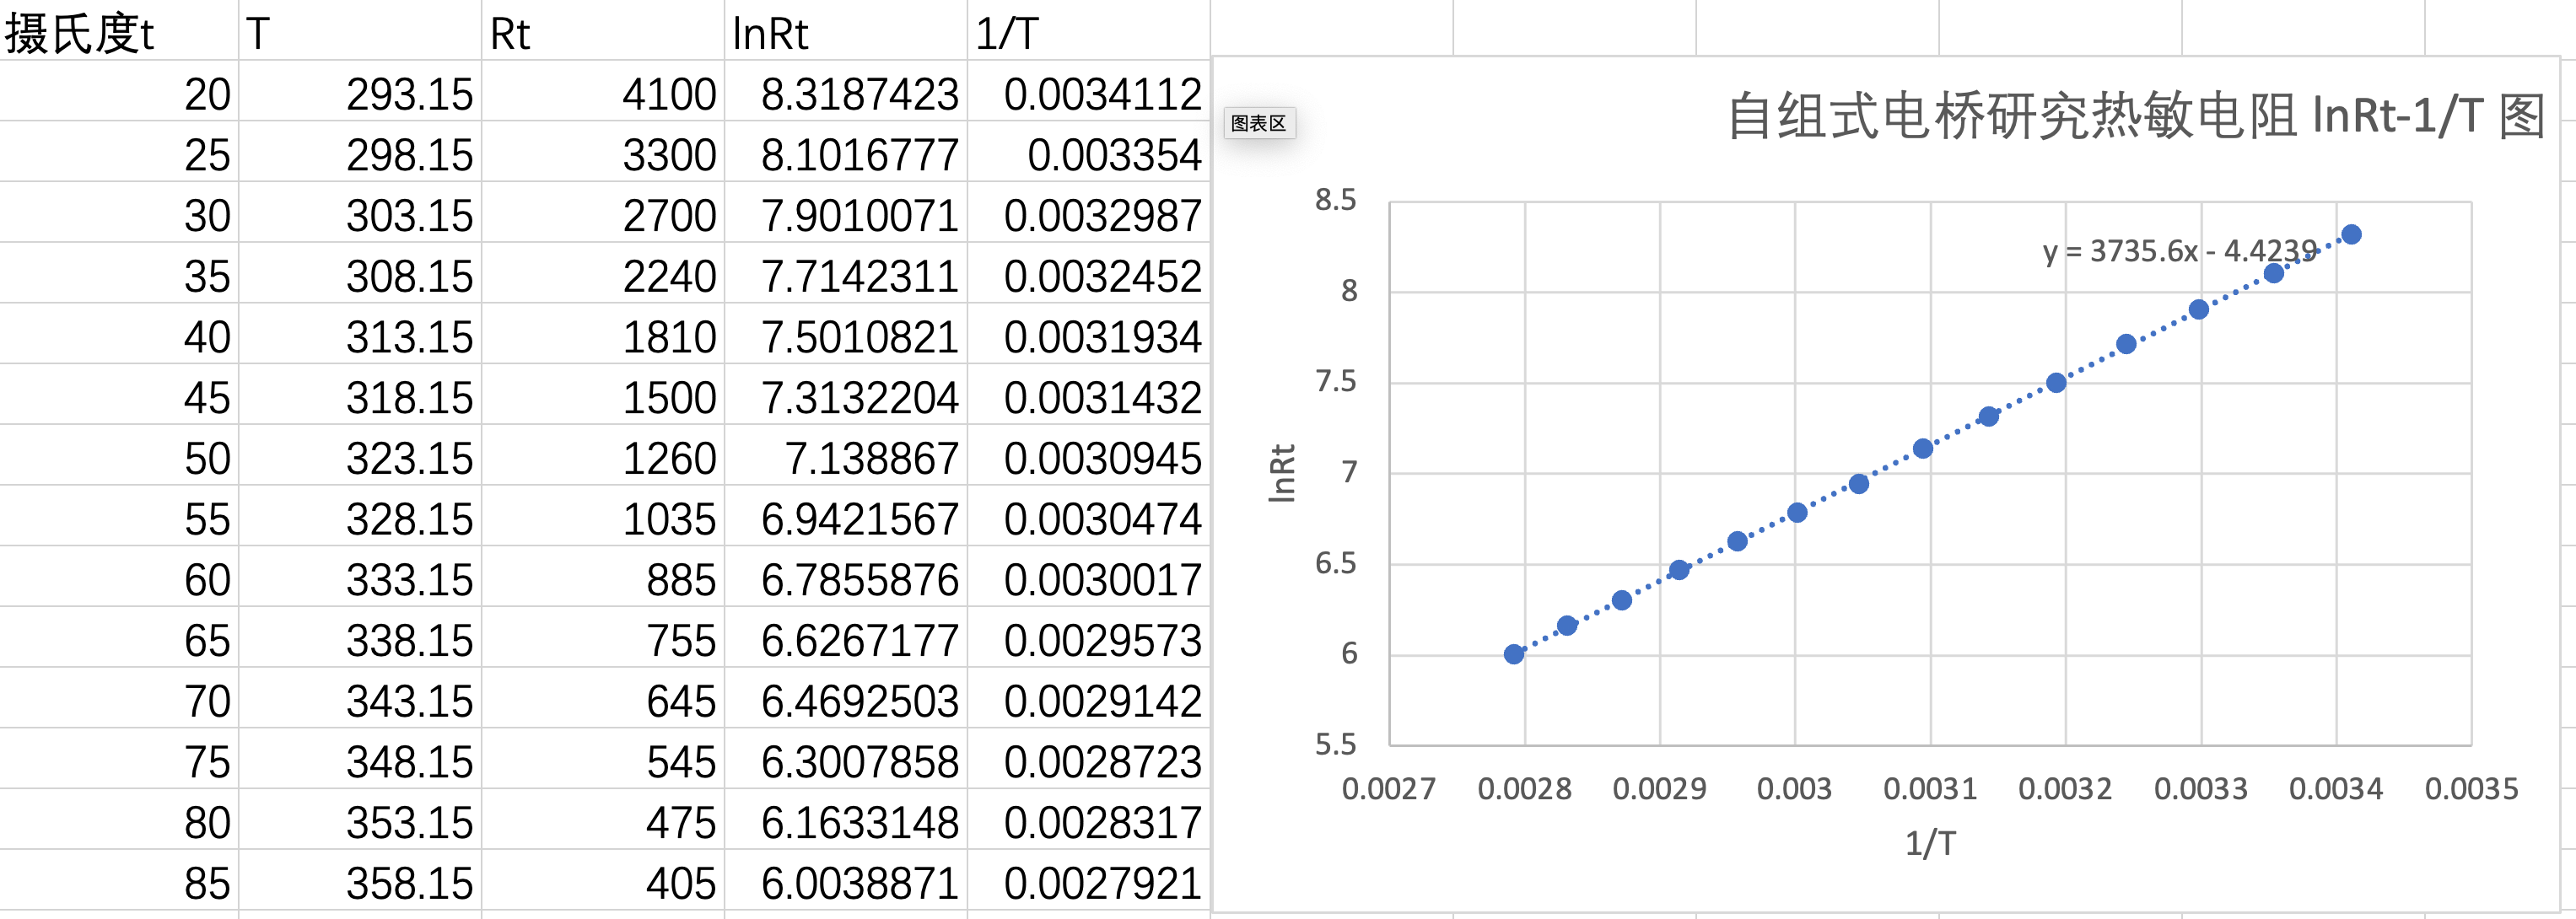
\includegraphics[width=0.8\textwidth]{6.png}
\end{figure}

(1)确定T趋于正无穷时热敏电阻的值:

截距A=-4.4239, 由:lna=A,  计算得:a=0.01198$\Omega$

(2)热敏电阻的材料常数B(单位:K):

材料常数B为拟合曲线的斜率:3735.6

(3)50摄氏度时的电阻温度系数$\alpha$(单位:1/K):

50+273.15=323.15K
由$\alpha=-\frac{B}{T^{2}}$=-0.0357




\section*{四、总结与分析}

\subsection*{思考题}

\subsubsection*{1.本实验的误差主要来源是什么?}
误差的主要来源是:(1)自热:热敏电阻有一个可变电阻一个小电流,因此须加热和它的热量消散在环境中。这个自加热效应的特征是热敏电阻的规格为扩散常数。热量是毫瓦的量级,因此对环境的影响是可以忽略的,在大多数情况下,但自加热效应显示为一个测量误差。耗散常数是功率来加热热敏电阻在空气中1摄氏度(1.8摄氏度)以上的环境温度下所需的量。较高的耗散常数是指测量结果会更准确。

(2)热时间常数:
热敏电阻有少量的质量,这是通常进行封装,用于机械保护。作为一个结果,将花费一定量的时间用于热敏电阻,以正确地测量温度时突然改变。热敏电阻器的热时间常数是时间,单位为秒,需要的热敏电阻来适应温度变化的63.2个百分点。例如,如果温度为50至60摄氏度改变10度,时间常数是读取56.32度所需的热敏电阻的时间。

(3)准确性:
由于自加热和时间常数测量的不准确,热敏电阻本身具有一定的耐受性在它的测量。这个误差可以在电阻或温度,要么在一个特定的点或在测量范围内的术语来表示一热敏电阻规格。误差的典型规范值可能是加/减1度在25度或+/-2度从零度到100度。在电阻方面,类似的规范可能加/减10欧姆。这种误差被添加到其它测量系统不准确。


\subsubsection*{2.利用半导体热敏电阻的温度特性,能否制作一只温度计?}
利用半导体热敏电阻的温度特性,可以制作一只温度计,根据温度和阻值对应的关系设计传感器,从而可以用于温度计的制作.


\subsection*{实验总结:}
热敏电阻是一种用于测量温度的电子元件,它的电阻值与周围环境温度成正比。在热敏电阻温度特性研究实验中,通常会测量热敏电阻在不同温度下的电阻值,并利用这些数据来研究热敏电阻的温度特性。
在实验中,首先需要准备所需的设备和材料,包括热敏电阻、电阻测量仪、加热器和温度计等。接下来,将热敏电阻放置在加热器上,并使用电阻测量仪测量热敏电阻的电阻值。同时,使用温度计测量热敏电阻周围的温度。这样,就可以记录下温度和电阻值之间的关系。
随着温度的升高,热敏电阻的电阻值也会随之增大。因此,通常可以画出温度和电阻值之间的曲线,从而更好地理解热敏电阻的温度特性。
在实验的最后,可以总结出热敏电阻的温度特性,包括其电阻值随温度变化的规律以及在不同温度下的电阻值变化范围等。此外,还可以对实验过程中出现的问题进行
分析,并提出改进建议。例如,在实验过程中,如果发现热敏电阻的电阻值变化幅度较小,可以考虑使用更灵敏的测量仪器或者选用具有更大温度灵敏度的热敏电阻来提高测量精度。

总的来说,热敏电阻温度特性线上研究实验是一个有趣且有意义的实验,既可以帮助我们了解热敏电阻的工作原理,又简化了实验的过程。


\end{document}